\documentclass[a4paper,10pt]{article}
%\usepackage[english]{babel}   % se si scrive in inglese
\usepackage[italian]{babel}       % se si scrive in italiano
\usepackage[T1]{fontenc}       % serve per la codifica delle lettere accentate (per evitare di scrivere \`e) 
\usepackage[utf8]{inputenc}   % serve per la codifica delle lettere accentate (per evitare di scrivere \`e)

\usepackage{graphicx}  % per includere le figure
\usepackage{rotating}   
\usepackage{lscape}
\usepackage{amsmath}
\usepackage{mathrsfs}
\usepackage[abs]{overpic}
\usepackage{color}
\usepackage{layout}
\usepackage[textwidth=16cm,textheight=24cm]{geometry} 

\usepackage{hyperref}

%% Definizione di nuovi commandi %%%
\newcommand{\latex}{\LaTeX}
\newcommand{\CP}{{\rm CP}}
\newcommand{\proton}{\ensuremath{p}}
\newcommand{\antiproton}{\ensuremath{\bar{p}}}
\newcommand{\acp}{\ensuremath{{\cal A}_{\CP}}}
\newcommand{\Lbppi}{\ensuremath{\Lambda_{b}^{0} \rightarrow p\pi^{-}}}
\newcommand{\aLbppi}{\ensuremath{\bar{\Lambda}_{b}^{0} \rightarrow \bar{p}\pi^{+}}}
\newcommand{\acplbppi}{\ensuremath{\acp(\Lbppi)}}
\newcommand{\lambdazero}{\ensuremath{\Lambda}}
\newcommand{\alambdazero}{\ensuremath{\bar{\Lambda}}}
\newcommand{\lambdazeroppi}{\ensuremath{\lambdazero \to \proton\pi^-}}
\newcommand{\alambdazeroppi}{\ensuremath{\bar{\lambdazero} \to \antiproton \pi^+}}

\newcommand{\pt}{\ensuremath{p_{\rm{T}}}}
\newcommand{\lxy}{\ensuremath{L_{\rm{T}}}}
\newcommand{\pdf}{\ensuremath{\wp}}

\newcommand{\mum}{\mbox{$\mu$m}}				%	um
\newcommand{\mus}{\mbox{$\mu$s}}
\newcommand{\tev}{\ensuremath{\mathrm{Te\kern -0.1em V}}}
\newcommand{\gev}{\ensuremath{\mathrm{Ge\kern -0.1em V}}}	%	GeV
\newcommand{\mev}{\ensuremath{\mathrm{Me\kern -0.1em V}}}	%	MeV
\newcommand{\kev}{\ensuremath{\mathrm{ke\kern -0.1em V}}}	%	keV
\newcommand{\massgev}{\mbox{\gev/$c^2$}}			%	GeV/c^2
\newcommand{\massmev}{\mbox{\mev/$c^2$}}			%	MeV/c^2
\newcommand{\pgev}{\mbox{\gev/$c$}}				%	GeV/c
\newcommand{\pmev}{\mbox{\mev/$c$}}				%	MeV/c

\newcommand{\note}[1]{\textcolor{red}{#1}}

%%%%%%%%%%%%%%%%%%%%%%%%%%
%%%%%% BEGIN DOCUMENT %%%%
%%%%%%%%%%%%%%%%%%%%%%%%%%
\begin{document}
\begin{flushright}             
\today
\end{flushright} 

\begin{center}
\Large{\bf Condizioni di lavoro di un contatore a scintillazione. }

\vspace*{1cm}                                 
\large{Michael De Nuccio, Fabio Spagliardi, Giacomi Vitali, Salvatore Zaza }\\ 
\vspace*{0.5cm}       
\vspace*{1.cm}
\end{center}

%{ \abstract  
%}


\section{Introduzione}
\label{sec:intro} 
Lo scopo dell'esperienza è quello di acquisire pratica con la strumentazione tipica del laboratorio e mettere a punto un sistema di tre rilevatori a scintillatore plastico. Si vuole inoltre valutare un adeguato punto di lavoro per poi stimare l'efficienza di uno dei tre rilevatori e la rilevanza del rumore rispetto al segnale vero.

%%%%%%%%%%%%%%%%%%%%%%%%%%%%%%%%%%%%%%%%%%%%%%%%%%%%%%%%%%%%%%%%%%%%%%%%%%%%%%%%
%%%%%%%%%%%%%%%%%%%%%%%%%%%%%%%%%%%%%%%%%%%%%%%%%%%%%%%%%%%%%%%%%%%%%%%%%%%%%%%%
%%%%%%%%%%%%%%%%%%%%%%%%%%%%%%%%%%%%%%%%%%%%%%%%%%%%%%%%%%%%%%%%%%%%%%%%%%%%%%%%
\section{Raggi cosmici}
Come si può facilmente evincere dal nome, i raggi cosmici sono raggi di varia natura provenienti dal cosmo; la loro origine non è ancora totalmente eviscerata, in particolare per quanto riguarda quelli ad altissima energia. La loro origine spazia dal Sole alle quasar ai confini dell'universo osservabile, e la loro natura è eterogenea: per lo più si tratta di protoni e particelle alfa, ma si hanno anche elettroni, positroni, fotoni, neutrini...

Al livello del mare però non si osservano tali specie: negli urti con le molecole dell'atmosfera si hanno varie reazioni con la conseguente produzione dei cosiddetti raggi cosmici secondari. Questi ultimi si dividono a loro volta in molli e duri a seconda della capacità di penetrazione, e se i primi vengono arrestati da pochi cm di materiale, i secondi possono penetrarvi anche per molti metri (con un range che ovviamente cresce al crescere del'energia).
I raggi cosmici secondari duri sono costituiti quasi interamente da muoni ($\mu^{\pm}$), e saranno questi che andremo per lo più a cercare coi nostri scintillatori plastici.

È quindi ovvio che siamo interessati ad una stima del numero di conteggi attesi.

Abbiamo dei valori "tabulati" per il flusso a livello del mare pari a\\

$\Phi\footnote{http://pdg.lbl.gov/2011/reviews/rpp2011-rev-cosmic-rays.pdf, pag.6;\\http://hyperphysics.phy-astr.gsu.edu/hbase/particles/muonatm.html}(\mu)\approx1$ cm$^{-1}$min$^{-1}$\\

Gli scintillatori adoperati hanno dimensioni $(55\pm1)$ cm $\times$ $(27\pm1)$ cm. La superficie risulta quindi $S=1485\pm61$ cm$^{2}$, con un conseguente rate di eventi attesi pari a:\\
\\
$R(\mu)\simeq(25\pm1)$ eventi/s
\\
\\(avendo assunto nullo l'errore sul numero "noto" di eventi e avendo propagato il resto in quadratura)

\section{Apparato Sperimentale}
\begin{figure}
\centering
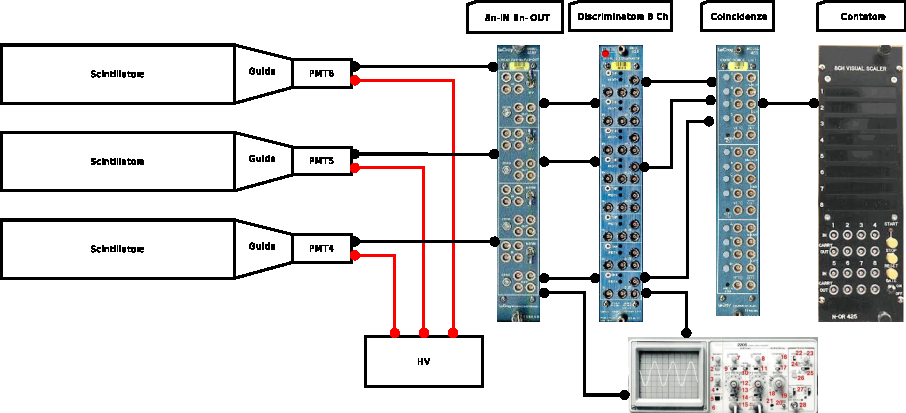
\includegraphics[width=\textwidth]{fig/apparato_sperimentale}
\caption{Schema generico dell'apparato sperimentale. I collegamenti varieranno a seconda delle misure effettuate come descritto nelle varie sezioni. La disposizione dei 3 PMT è fedele alla realtà. }
\label{fig:apparato}
\end{figure}

In figura \ref{fig:apparato} è schematizzano l'apparato sperimentale. E' composto da tre scintillatori collegati tramite una guida d'onda ad un fotomoltiplicatore (PMT). Faremo riferimento ai 3 tramite il numero associato al loro PMT (come in figura).

I PMT sono alimentati tramite un modulo dell'alta tensione (HV). 

Per l'osservazione e l'acquisizione dei segnali dai PMT abbiamo utilizzato i seguenti strumenti elettronici:
\begin{itemize}
\item multimetro digitale;
\item oscilloscopio a 2 canali;
\item modulo FAN-IN FAN-OUT per lo smistamento dei segnali;
\item discriminatore NIM a 8 canali;
\item diversi moduli per il delay dei segnali;
\item un modulo NIM per le coincidenze;
\item un contatore digitale NIM con timer;
\item cavi di diversa lunghezza con impedenza standardizzata di 50 $\Omega$.
\end{itemize}


\label{sec:apparato} 

\subsection{Scintillatore Plastico}
Uno scintillatore plastico è composto da una lastra di materiale plastico in cui è dissolta una sostanza organica capace di emettere fotoni quando viene attraversato da una particella ionizzante. Si tratta di rilevatori veloci che si prestano bene ad essere utilizzati per realizzare contatori: infatti i tempi tipici sono dell'ordine del nanosecondo. La luce emessa dalla diseccitazione degli elettroni eccitati dal passaggio della particella ionizzante si propaga all'interno del rivelatore attraverso il meccanismo della riflessione totale. Il fotone emesso non viene riassorbito grazie al principio di Franck-Condon. La luce si riflette fino all'estremità dello scintillatore dove continua a propagarsi in una guida di luce, la quale permette di raccordare la superficie del rivelatore con il fotomoltiplicatore.

Nel nostro caso i tre scintillatori sono ricoperti da scotch nero. Ciò permette di isolare dalla luce ambientale e, allo stesso tempo, si riesce a lasciare uno strato d'aria tra la superficie esterna del rilevatore e lo scotch: ciò è ottimale per avere riflessione totale alle superficie.

\subsection{PhotoMultiplier Tube (PMT)}
Ognuno dei tre scintillatori è collegato ad un fotomoltiplicatore. Non si dispone di un datasheet per il modello utilizzato.

Un fotomoltiplicatore, in generale, è formato da una sequenza di elettrodi (detti dinodi, la cui geometria può essere molto variabile). Agli estremi di questa sequenza sono presenti un anodo e un catodo. Il fotone che esce dallo scintillatore si trova ad interagire con il catodo tramite effetto fotoelettrico (effetto dominante considerate le energie a cui si lavora, ovvero qualche KeV). Grazie al campo elettrico introdotto tramite la differenza di potenziale tra catodo e anodo i primi, e relativamente pochi, elettroni prodotti vengono accelerati e, mediante ionizzazione per urto con gli elettrodi interposti, si innesca un fenomeno a cascata che porta ad aumentare il numero di elettroni che vengono via via accelerati. Per essere più quantitativi si può considerare il numero di elettroni che vengono estratti ad ogni elettrodo: $\delta=2\div 5$; il guadagno totale in elettroni sarà quindi $G=\delta ^N$ dove $N$ è il numero totale di dinodi. Solitamente il catodo viene messo a massa e l'anodo viene tenuto ad una tensione elevata (1000-2000 $V$); tramite un partitore di tensione i dinodi vengono mantenuti a tensioni intermedie opportune. Alla fine di questo processo si osserva un segnale elettrico macroscopico.

Per stimare l'ampiezza di questo segnale si può ricorrere ad un calcolo veloce: tipicamente si trova che il numero di fotoni prodotti è $2\times 10^{4}$ per centimento di spessore del rilevatore. Facendo un calcolo indicativo si ottiene il numero di fotoni che effettivamente giungono al fotomoltiplicatore è circa $1400$, numero ottenuto considerando l'efficacia di raccolta della luce da parte della guida, il rapporto tra le interfacce di scintillatore e PMT e l'attenuazione esponenzialmente decrescente con la distanza, durante la propagazione. Si definisce il parametro $\eta$, detto "efficienza quantica", come la frazione di fotoni che riescono a fare un effetto fotoelettrico efficace. Di conseguenza, moltiplicando per $\eta$, si ottengono 350 fotoelettroni. Se si considera come guadagno tipico di un PMT $G=\delta ^N=3^{12}=5 \times 10^5$ si ottengono all'anodo $1,8 \times 10^8$ elettroni, ovvero una carica di 29 pC. Considerato che questa carica è spalmata in un intervallo temporale dell'ordine di 10 ns si ottiene un'intensità di corrente $I=3$ mA che equivale, con una resistenza standardizzata all'anodo di $50\ \Omega$, ad un segnale dell'ordine di 150 mV. Questo tipo di segnale è facilmente visualizzabile e misurabile tramite un oscilloscopio.



\subsection{Elettronica di Front-End}
L'elettronica di Front-End è composta dai moduli, digitali e analogici, indicati sopra. Il segnale in uscita dal fotomoltiplicatore è stato tipicamente mandato al modulo per il delay regolabile dei segnali. L'uscita del modulo per il delay veniva inviata al modulo FAN-IN FAN-OUT per lo smistamento dei segnali, facendo attenzione alle terminazioni. Questa configurazione iniziale permette di ritardare a piacimento il segnale e a formarne quattro copie che possono essere mandatie ai vari moduli o analizzanti con l'oscilloscopio. Un segnale veniva poi inviato al discriminatore il quale, una volta impostata la soglia, converte il segnale in ingresso in un segnale digitale secondo la logica NIM. Il modulo che abbiamo utilizzato permette sia di regolare il livello del discriminatore, sia la durata dell'impulso (piatto) associato. La scelta di questi parametri verrà specificata nel seguito. A questo punto si è usato il contatore digitale NIM con timer regolabile per contare gli impulsi digitali in uscita dal discriminatore. Tutto quanto detto verrà fatto per ogni singolo fotomoltiplicatore utilizzato. 






%%%%%%%%%%%%%%%%%%%%%%%%%%%%%%%%%%%%%%%%%%%%%%%%%%%%%%%%%%%%%%%%%%%%%%%%%%%%%%%%
%%%%%%%%%%%%%%%%%%%%%%%%%%%%%%%%%%%%%%%%%%%%%%%%%%%%%%%%%%%%%%%%%%%%%%%%%%%%%%%%
%%%%%%%%%%%%%%%%%%%%%%%%%%%%%%%%%%%%%%%%%%%%%%%%%%%%%%%%%%%%%%%%%%%%%%%%%%%%%%%%


\section{Ricerca del punto di lavoro}
\label{sec:puntodilavoro} 
\subsection{Calibrazione del discriminatore e del contatore}
Abbiamo preventivamente testato l'affidabilità del discriminatore, con particolare attenzione alla proporzionalità fra la soglia di threshold effettiva e la tensione rilevata sul pin predisposto. Era atteso, stando al data sheet, un rapporto 1:10.

Per far ciò ci siamo muniti di un impulsatore al fine di avere a disposizione una tensione regolabile. Visionata essa con l'oscilloscopio si è mandato tale segnale anche al discriminatore, mandando pure il segnale di quest'ultimo all'oscilloscopio.

Partiti dalla threshold minima ($\approx320$ mV misurati al pin) l'abbiamo aumentata lasciando inizialmente invariata l'ampiezza dell'onda quadra proveniente dall'impulsatore, $\approx80$ mV, fino a che non è scomparso il segnale proveniente dal discriminatore. Notato il voltaggio segnato dal pin abbiamo poi aumentato progressivamente l'ampiezza dell'onda quadra e continuato ad aumentare la threshold fino a che nuovamente il segnale dal discriminatore non scompariva. Testata la diretta proporzionalità entro la zona nella quale contavamo di operare abbiamo accertato il rapporto 1:10 entro un $\sim2\%$.
\\Per quanto concerne la verifica della frequenza di pulsazione del contatore abbiamo semplicemente attaccato l'uscita del contatore stesso all'oscilloscopio ed osservato la forma d'onda e la frequenza della stessa. Essa è risultata essere, come atteso, un'onda quadra, e la frequenza era di $1000\pm$ Hz per tutte le durate temporali scandagliate: 1 s, 10 s, 100 s, che sono state quelle poi adoperate nel corso dell'esperienza.

\subsection{Osservazioni preliminari}
Inizialmente abbiamo alimentate il PMT4 con una tensione di 1.700 V, osservando un assorbimento in corrente di 0,693 mA. Collegando il segnale all'oscilloscopio ed impostando una soglia di trigger di 30 mV abbiamo visualizzato impulsi della durata dai 25 ai 31 ns, di ampiezza molto variabile dai 30 ai 750 mV, ad una frequenza dell'ordine dei kHz.


Quindi abbiamo collegato il PMT ad un contatore tramite un discriminatore, impostato con una soglia a 50mV e una larghezza del segnale di uscita di 40ns. In questo modo abbiamo preso le misure mostrate nel grafico \ref{fig:none}, che mostra una netta differenza nei conteggi in caso di luce accesa o spenta, segnalandoci la possibile presenza di imperfezioni nella copertura esterna.


Nelle prossime misure abbiamo cercato di limitare questo effetto ricoprendo l'apparato con un panno nero.


Per le misure dei conteggi abbiamo scelto di adottare un tempo di acquisizione di 100s, risultato come compromesso fra l'avere una quantità di dati adeguata sia ai tempi di lavoro necessari ad effettuare praticamente la presa dati sia per avere delle fluttuazioni sui dati stessi abbastanza piccole, avendo le fluttuazioni relative un andamento del tipo $1\over{\sqrt{N}}$, con N=numero di misure.
%%%%%%%%%%%%%%%%%%%%%%%%%%%%%%%%%%%%%%%%%%%%%%%%%%%%%%%%%%%%%%%%%%%%%%%%%%%%%%%%
%%%%%%%%%%%%%%%%%%%%%%%%%%%%%%%%%%%%%%%%%%%%%%%%%%%%%%%%%%%%%%%%%%%%%%%%%%%%%%%%
%%%%%%%%%%%%%%%%%%%%%%%%%%%%%%%%%%%%%%%%%%%%%%%%%%%%%%%%%%%%%%%%%%%%%%%%%%%%%%%%
\subsection{Curva in funzione della tensione di alimentazione}
\begin{figure}
\centering
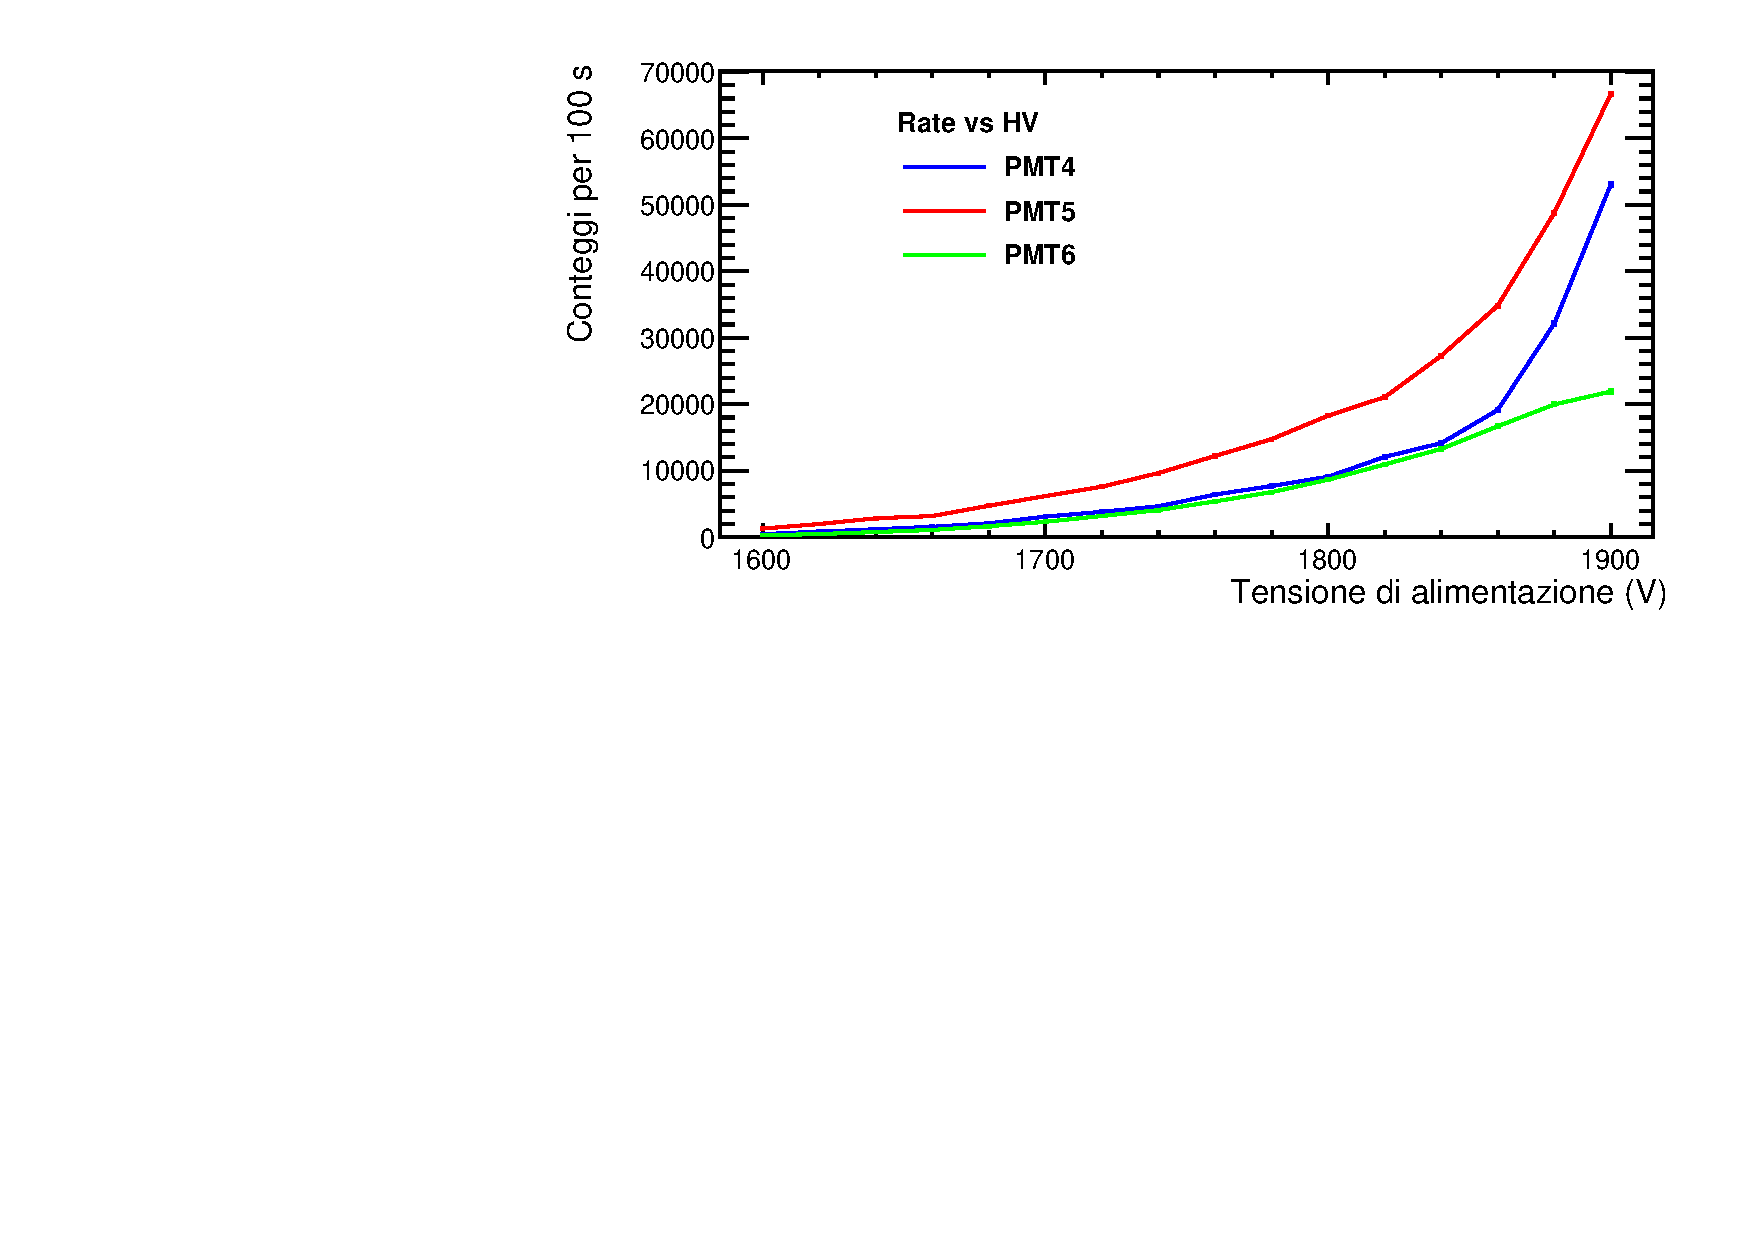
\includegraphics[width=\textwidth]{fig/rate-hv}
\caption{Numeri di conteggi ogni 100 secondi al variare della tensione di alimentazione dei PMT.}
\label{fig:rate-hv}
\end{figure}
Abbiamo alimentato tutti e 3 PMT con una tensione variabile da 1600 a 1900 mV. Abbiamo collegato il segnale dei 3 PMT ad un contatore passando attraverso un discriminatore per il conteggio degli impulsi.


Per questa misura abbiamo impostato la minima soglia possibile per il discriminatore, ovvero 32~mV, allo scopo di ottenere una stima conservativa. 
Abbiamo anche impostato una larghezza del segnale di uscita del discriminatore di 40 ns: in questo modo abbiamo eliminato la possibilità di avere conteggi accidentali causati dai piccoli rimbalzi successivi al segnale principale. 

Il grafico in figura~\ref{fig:rate-hv} mostra il numero dei conteggi in funzione della tensione di alimentazione. Si può osservare come i PMT 4 e 6 mostrano un andamento molto simile mentre il PMT 5 presenta un tasso di conteggi più elevato.

Da queste misure risulta difficile individuare un plateau, ma le abbiamo utilizzate in seguito per scegliere punti di lavoro che presentassero una variazione minima del tasso dei conteggi in funzione di variazioni della tensione di alimentazione.

Il numero dei conteggi è molto variabile e non ci permette di stabilire una relazione col numero di raggi cosmici attesi. D'altra parte ci aspettiamo che un singolo scintillatore presenti una quantità di conteggi dovuti al rumore di fondo molto maggiore del numero di conteggi dovuti al passaggio di particelle ionizzanti, ed è per questo che ci aspettiamo tassi di conteggi molto elevati.

\subsection{Calibrazione delle coincidenze}
\begin{table}
\centering
\begin{tabular}{|c|c|c|c|}
\hline
\textbf{HV (V)} & \textbf{PMT4 (Conteggi)} & \textbf{PMT6 (Conteggi)} & \textbf{Coincidenze casuali attese (Hz)} \\
\hline 
1600 & 451 & 281 & 1.27e-06 \\
\hline
1620 & 832 & 470 & 3.91e-06 \\
\hline
1640 & 1189 & 772 & 9.18e-06 \\
\hline
1660 & 1562 & 1088 & 1.70e-05 \\
\hline
1680 & 2084 & 1654 & 3.45e-05 \\
\hline
1700 & 3095 & 2313 & 7.16e-05 \\
\hline
1720 & 3815 & 3189 & 1.22e-04 \\
\hline
1740 & 4644 & 4074 & 1.89e-04 \\
\hline
1760 & 6408 & 5385 & 3.45e-04 \\
\hline
1780 & 7698 & 6775 & 5.22e-04 \\
\hline
1800 & 9093 & 8648 & 7.86e-04 \\
\hline
1820 & 12081 & 10945 & 1.32e-03 \\
\hline
1840 & 14148 & 13284 & 1.88e-03 \\
\hline
1860 & 19136 & 16686 & 3.19e-03 \\
\hline
1880 & 32146 & 19968 & 6.42e-03 \\
\hline
1900 & 53110 & 21913 & 1.16e-02 \\
\hline

\end{tabular} 
\caption{Calcolo delle coincidenze casuali attese sul numero di conteggi acquisiti per 100 secondi al variare della tensione di alimentazione}
\label{tab:random_coincidence}
\end{table}

\begin{figure}
\centering
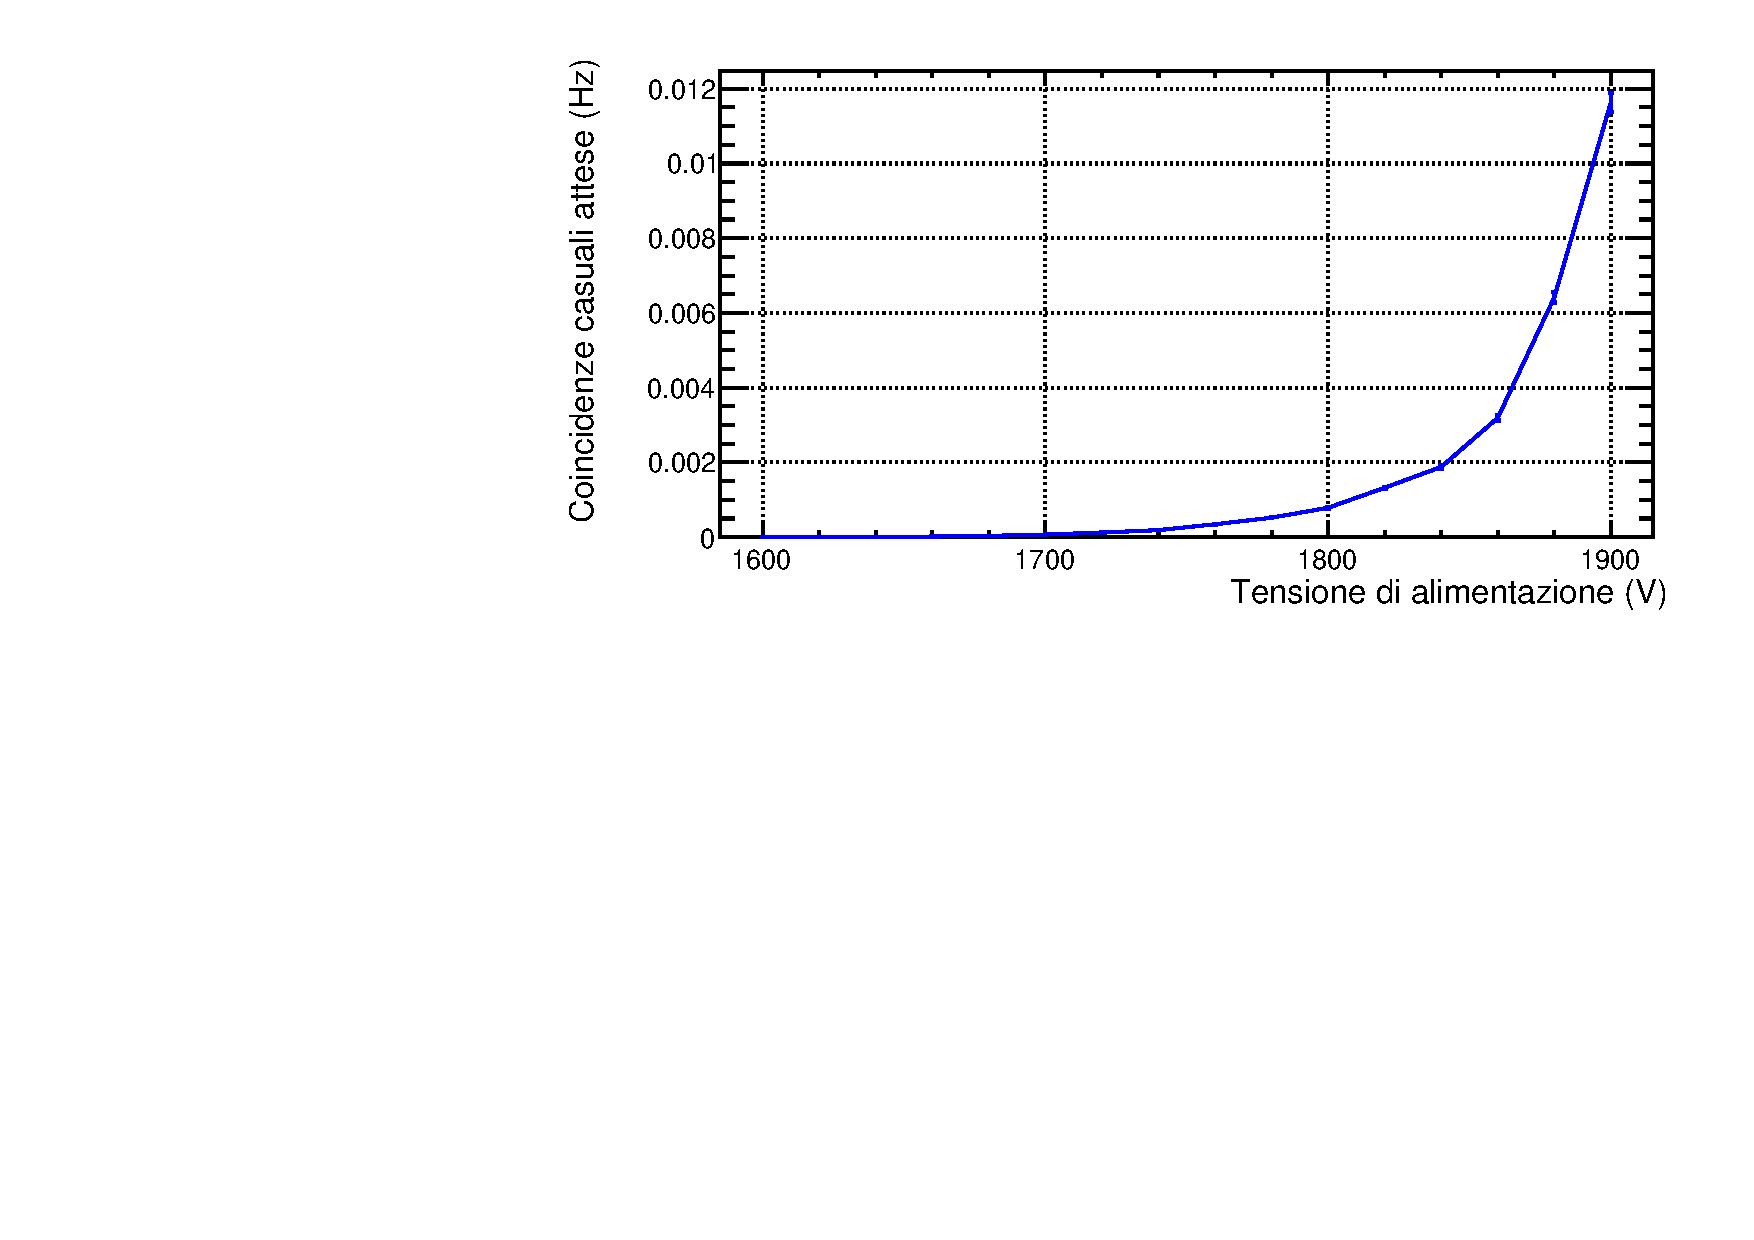
\includegraphics[width=\textwidth]{fig/random_coincidence}
\caption{Calcolo delle coincidenze casuali attese per i PMT4 e 6 in funzione della tensione di alimentazione, fatto sui conteggi acquisiti per 100 secondi. Vedi tabella~\ref{tab:random_coincidence}.}
\label{fig:random_coincidence}
\end{figure}

\begin{figure}
\centering
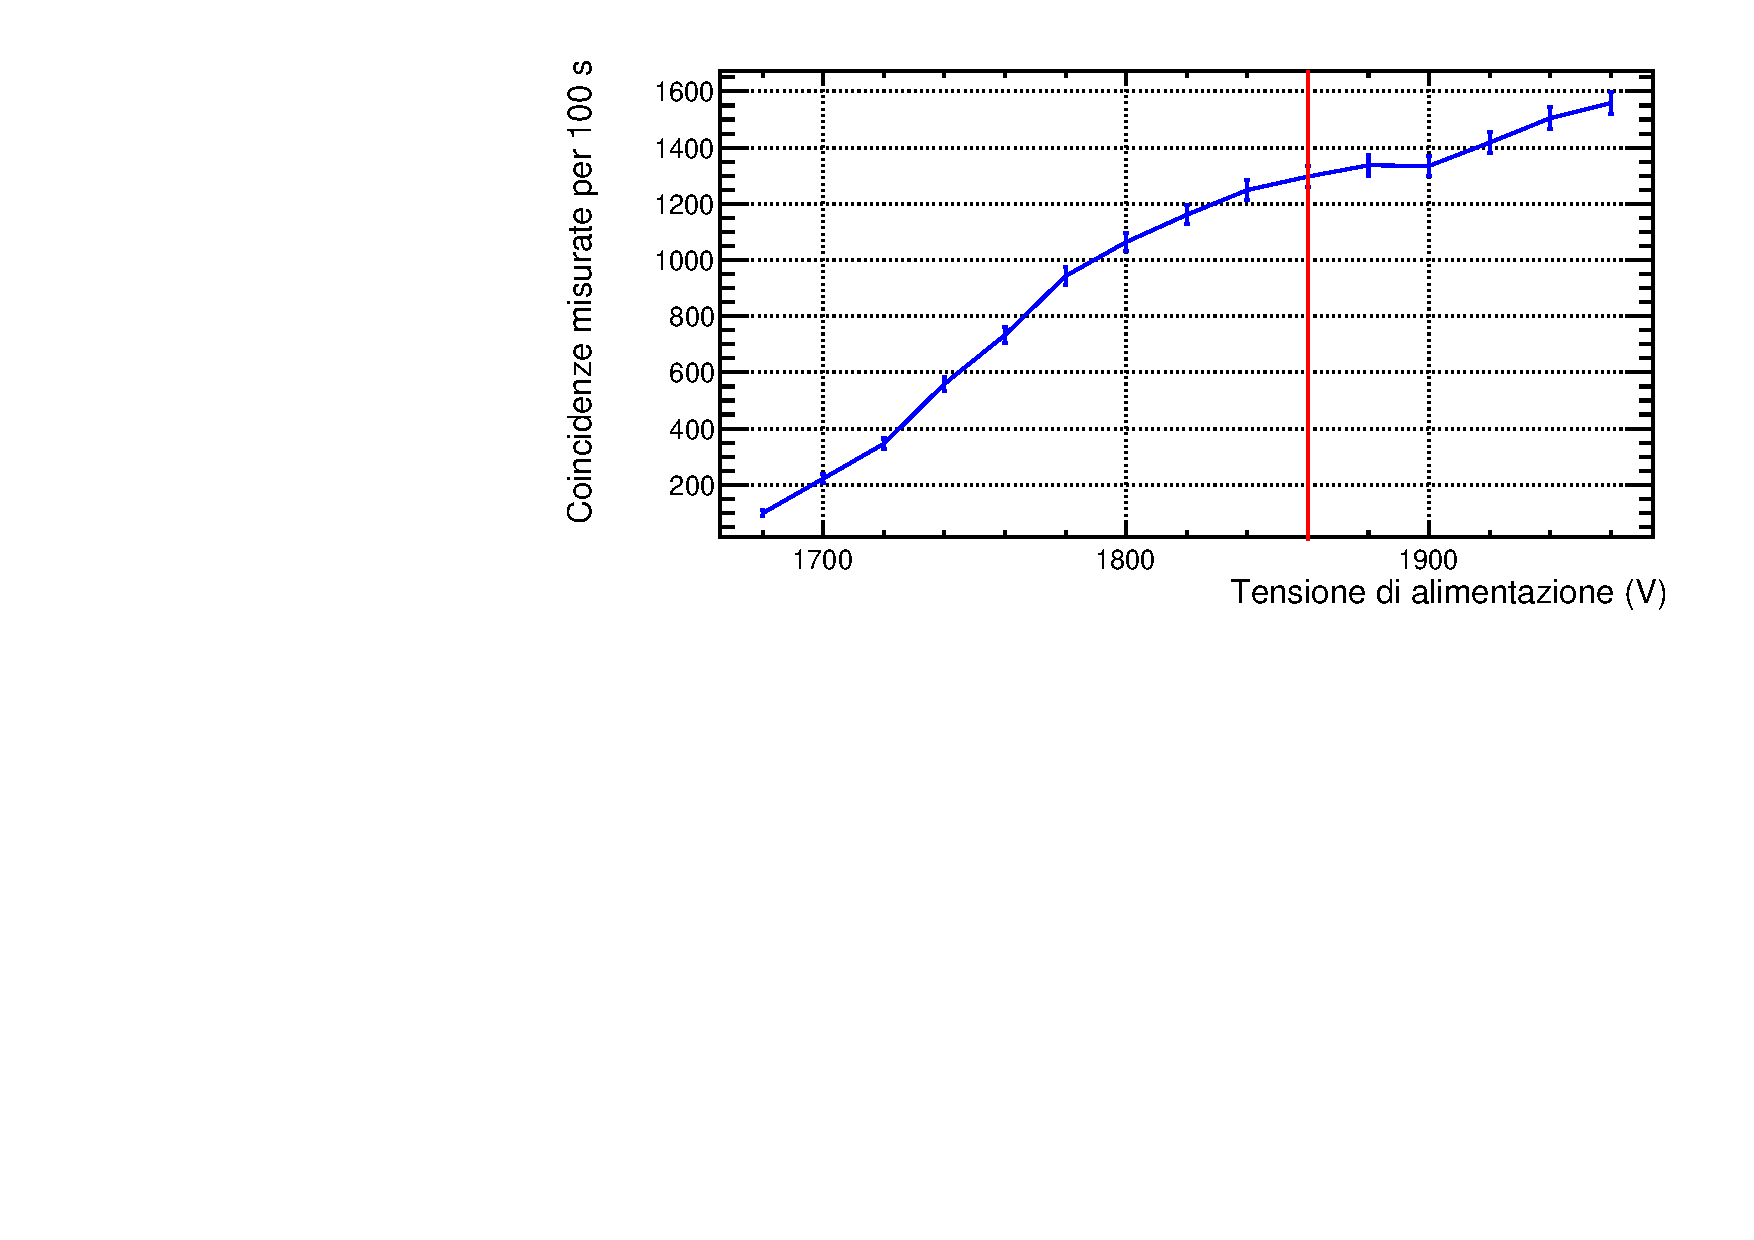
\includegraphics[width=\textwidth]{fig/coincidence}
\caption{Misura delle coincidenze per i PMT4 e 6 in funzione della tensione di alimentazione. Acquisizione di 100 secondi. Data la natura Poissoniana della distribuzione l'errore sui conteggi è stato calcolato come $\sqrt{R}$. Evidenziato in rosso il punto di ascisse 1860 V.}
\label{fig:coincidence}
\end{figure}

Utilizzando i dati in tabella~\ref{tab:random_coincidence}, abbiamo calcolato il tasso di coincidenze casuali attese tra il PMT 4 e 6.

Osservando il grafico in figura~\ref{fig:random_coincidence} ci siamo assicurati che mantenendoci al di sotto di una soglia di alimentazione di 1900 V il numero di coincidenze casuali non influisce in maniera significativa sul conteggio di coincidenze reali che ci aspettiamo.  

Il calcolo è stato effettuato considerando una larghezza del segnale del discriminatore di 50 ns, e utilizzando la formula:
\begin{equation}
R_{c} = R_{4} \times R_{6} \times \Delta t
\label{eq:random_coincidence}
\end{equation}
Con $R_{c}$ uguale al tasso di coincidenze casuali attese, $R_{4,6}$ i conteggi al secondo misurati sul PMT 4 e 6, e $\Delta t = 100$~ns (pari alla somma della larghezza del segnale dei due discriminatori collegati in serie ai PMT) .

Gli errori sui conteggi sono stati calcolati utilizzando la formula:
\begin{equation}
\sigma_{R_{c}} = R_{c} \times{\sqrt{\frac{1}{R_{4}} + \frac{1}{R_{6}} + \left( \frac{\sigma_{t}}{\Delta t} \right)^2}  }
\end{equation}
con $\sigma_{t} = 5$~ns, mentre i conteggi seguono la distribuzione di Poisson e di conseguenza assegnamo $\sqrt{R}$ come incertezza.

A questo punto abbiamo effettuato la misura delle coincidenze in funzione della tensione di alimentazione sui PMT 4 e 6, per trovare un punto di plateau da poter utilizzare per la misura di efficienza del PMT 5.
In questo caso abbiamo deciso di impostare una soglia di 60 mV per limitare il rumore mantenendo comunque il segnale ad un'ampiezza misurabile. 

I risultati di questa misura si possono osservare in figura~\ref{fig:coincidence}. \`E ben visibile un plateau ad una tensione di alimentazione di circa 1860 V.	


\subsubsection{Curva di cavo}
\begin{figure}
\centering
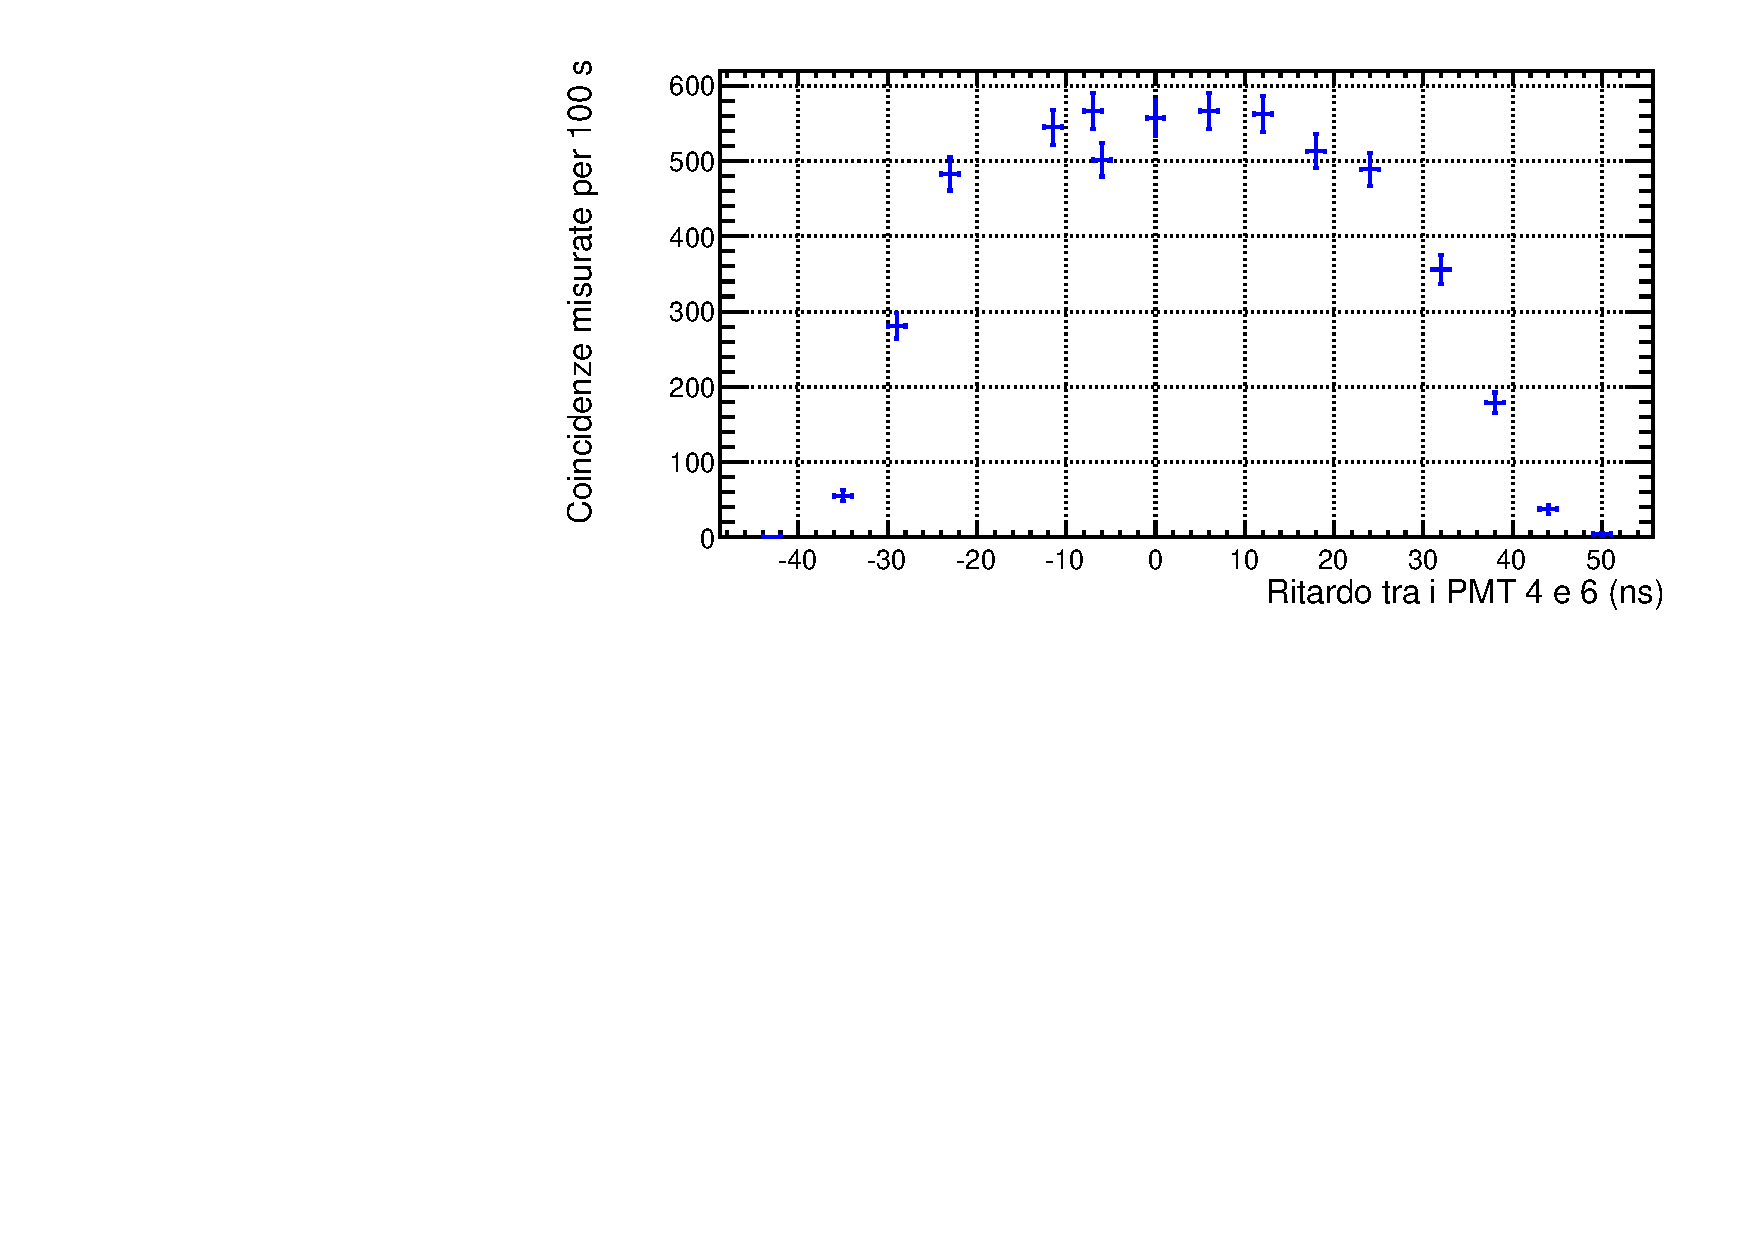
\includegraphics[width=\textwidth]{fig/delay_curve}
\caption{Misura delle coincidenze per i PMT4 e 6 in funzione del ritardo di cavo. Acquisizione di 100 secondi.}
\label{fig:delay_curve}
\end{figure}
Abbiamo realizzato una curva di cavo tra i PMT4 e 6 per assicurarci che i segnali provenienti dai due PMT giungano al modulo delle coincidenze con un ritardo inferiore alla larghezza dei segnali in uscita dei due discriminatori impostata a $t = 50$ ns. 

In figura~\ref{fig:delay_curve} si possono osservare i risultati. La forma quadra del grafico è compatibile con le nostre attese, la larghezza del plateau ci consente di tenerci al riparo da possibili errori dovuti ad oscillazioni nella larghezza del segnale di uscita dei discriminatori. 

Il fatto che la curva sia leggermente spostata verso destra rispetto allo zero potrebbe suggerire l'idea di aggiungere un po' di ritardo tra i due segnali, ma non lo abbiamo comunque ritenuto necessario.
\subsubsection{Misura delle coincidenze casuali}
Abbiamo effettuato una misura delle coincidenze casuali aumentando il ritardo tra i segnali del PMT 4 e 6 ben oltre i valori suggeriti dalla curva in figura~\ref{fig:delay_curve}, in modo da abbattere il numero di coincidenze reali. Considerando che ci aspettavamo un numero di coincidenze casuali molto basse, abbiamo acquisito i dati per un periodo molto più lungo delle precedenti misure.

Il risultato ottenuto visibile in tabella~\ref{tab:random_coincidence_mesured}. Otteniamo un risultato di un ordine di grandezza superiore la nostra stima, quindi è possibile che in questo caso abbiamo sottostimato l'errore. 

\begin{table}
\centering
\begin{tabular}{|c|c|c|c|c|}
\hline 
tempo (s) & Coincidenze & Tasso Coincidenze Casuali (Hz) & Tasso atteso (Hz) \\ 
\hline 
24450 & 1391 & 0.057 & 0.0035\\ 
\hline 
\end{tabular} 
\caption{Misura coincidenze casuali tra PMT 4 e 6, alimentati entrambi con una tensione di 1870 V e con una soglia di 70 mV. Il tasso atteso è stato calcolato secondo la formula~\ref{eq:random_coincidence} .}
\label{tab:random_coincidence_mesured}
\end{table}

\section{Misura dell'efficienza}
L'efficienza ($\epsilon_x$) di un terzo PMT può essere ricavata considerando che $\epsilon_1\times \epsilon_2=N_{4,6}/N_r$ e $\epsilon_1\times \epsilon_2\times \epsilon_3=N_{4,5,6}/N_r$ (dove $N_r$ è il numero di eventi reali, $N_{4,6}$ e $N_{4,5,6}$ sono rispettivamente le coincidenze dei PMT 4 e 6, e dei PMT 4, 5 e 6; facendo il rapporto tra queste due relazioni si ottiene infatti $\epsilon_3=N_{4,5,6}/N_{4,6}$. Abbiamo scelto di ottenere l'efficienza del PMT 5, cioè quello centrale nella nostra configurazione, in modo tale da annullare errori dovuti all'accettanza geometrica, poichè chiaramente se una particella passa nei PMT esterni, determinando un segnale, dovrà farlo necessariamente anche nel terzo, ipotizzando ovviamente una traiettoria rettilinea. Quindi è stata fatta variare la tensione di alimentazione del PMT 5 in modo tale da ottenere una curva di efficienza assoluta, ottenendo i risultati osservabili nel grafico~\ref{fig:efficiency}.

I valori delle tensioni applicate ai PMT 4 e 6 sono quelle considerate ottimali nei punti precedenti, mentre per ogni punto del grafico la presa dati ha avuto una durata di $t=100s$ e la soglia del discriminatore è stata fissata a 60mV per tutti i PMT.
\subsection{Risultati}
Dal grafico~\ref{fig:efficiency} si vede chiaramente che, aumentando la tensione, l'efficienza aumenta tendendo a 1, come ci si aspetterebbe, dato che il PMT conta più eventi veri mentre le coincidenze casuali rimangono trascurabili, come si è visto al punto precedente. Infatti attorno a valori di tensione di alimentazione di $V=1860V$ si ha un'efficienza $\epsilon_3=0.9846\pm0.8$. L'errore è stato calcolato considerando una distribuzione poissoniana degli eventi.

\begin{figure}
	\centering
	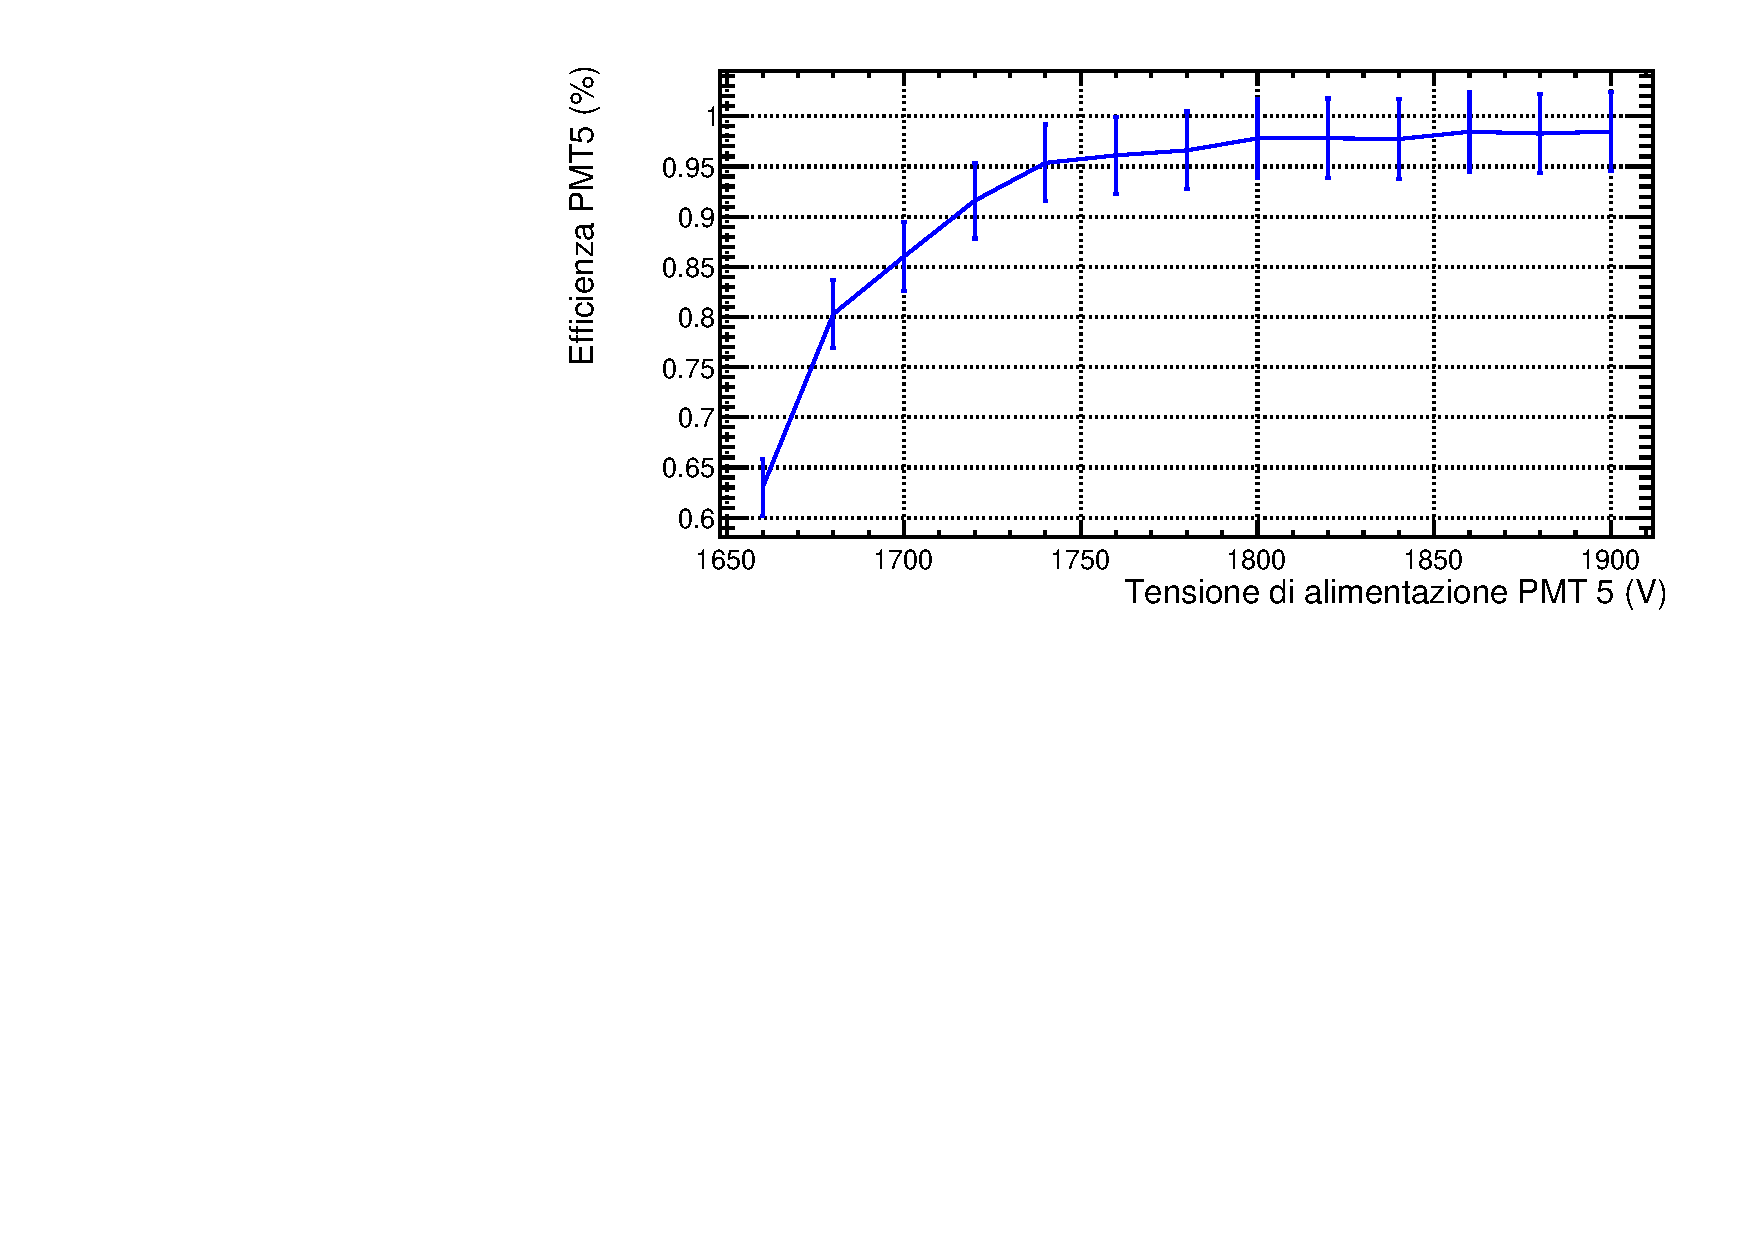
\includegraphics[width=\textwidth]{fig/efficiency}
	\caption{Misura dell'efficienza del PMT centrale in funzione della tensione di alimentazione dello stesso.}
	\label{fig:efficiency}
\end{figure}

\label{sec:efficienza} 

%%%%%%%%%%%%%%%%%%%%%%%%%%%%%%%%%%%%%%%%%%%%%%%%%%%%%%%%%%%%%%%%%%%%%%%%%%%%%%%%
%%%%%%%%%%%%%%%%%%%%%%%%%%%%%%%%%%%%%%%%%%%%%%%%%%%%%%%%%%%%%%%%%%%%%%%%%%%%%%%%
%%%%%%%%%%%%%%%%%%%%%%%%%%%%%%%%%%%%%%%%%%%%%%%%%%%%%%%%%%%%%%%%%%%%%%%%%%%%%%%%

%\appendix


\end{document}